\graphicspath{ {Figures/Pileup/Energies/} {Figures/Main/} {Figures/ResidualsFFT/} {Figures/FitStartScans/} {Figures/PerCalo/} }

\chapter{Analysis Results}

\section{Pre-corrected and corrected energy and time spectra}

\begin{figure}[h]
	\centering
	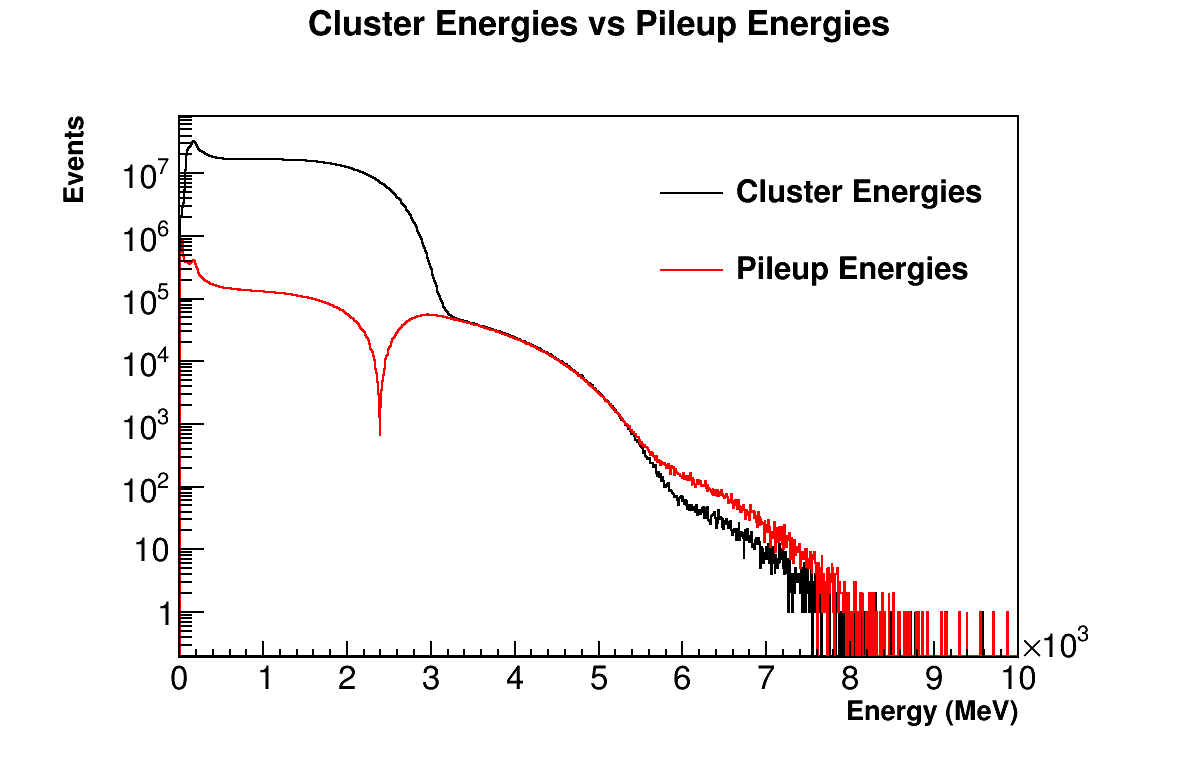
\includegraphics[width=\textwidth]{ClusterEnergiesVsPileupEnergies}
    \caption[ClusterEnergiesVsPileupEnergies]{Cluster energies in black are plotted vs pileup energies in red, for all calorimeters added together. At energies below about 2.4 GeV the pileup spectrum goes negative. In this plot the absolute value of the pileup energies is plotted, and a spike at about 2.4 GeV can be seen as a consequence of this. Due to the triplets and contamination in the pileup spectrum, the red and black curves can be seen to diverge at high energies.}    
    \label{fig:ClusterEnergiesVsPileupEnergies}
\end{figure}

\begin{figure}[]
\centering
    \begin{subfigure}[]{0.8\textwidth}
	    \centering
		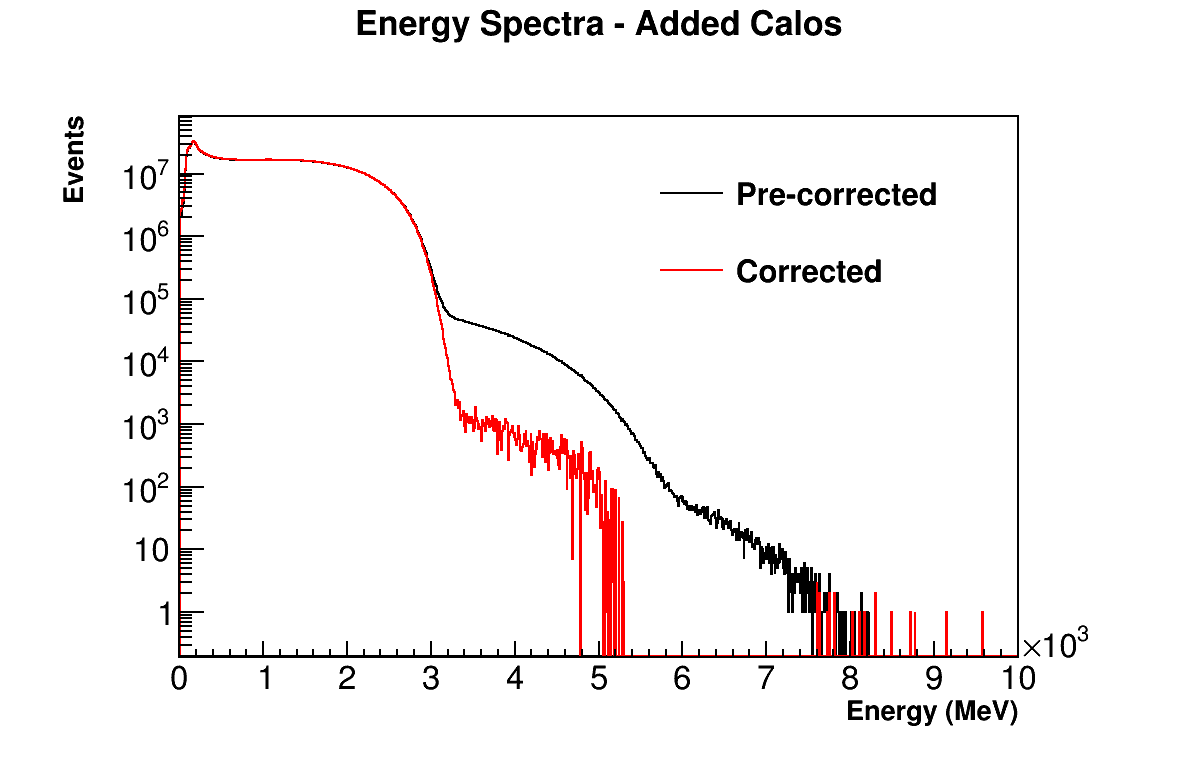
\includegraphics[width=\textwidth]{AddedEnergies}
	    \caption{Log scale - the corrected energy spectrum goes negative around 5 GeV.}
    \end{subfigure}% %you need this % here to add spacing between subfigures
    \vspace{1cm}
    \begin{subfigure}[]{0.8\textwidth}
	    \centering
		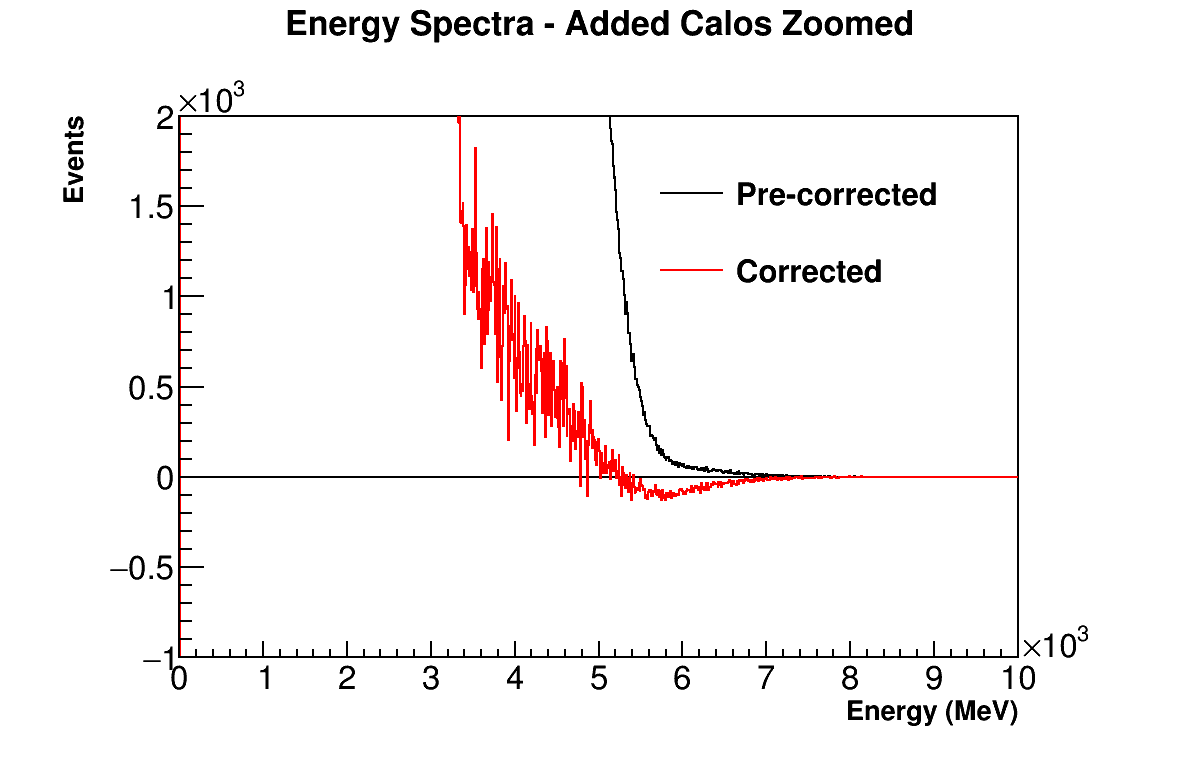
\includegraphics[width=\textwidth]{AddedEnergiesZoomed}
	    \caption{Linear scale - zoomed in to show the shape.}
    \end{subfigure}
\caption[AddedEnergies]{Plots for the pre-corrected and corrected energy spectra are shown, all calorimeters added together. Because the triplets and contamination are not accounted for, the corrected energy spectrum does not lie exacltly along zero.}
\label{fig:AddedEnergies}
\end{figure}

\begin{figure}[]
	\centering
	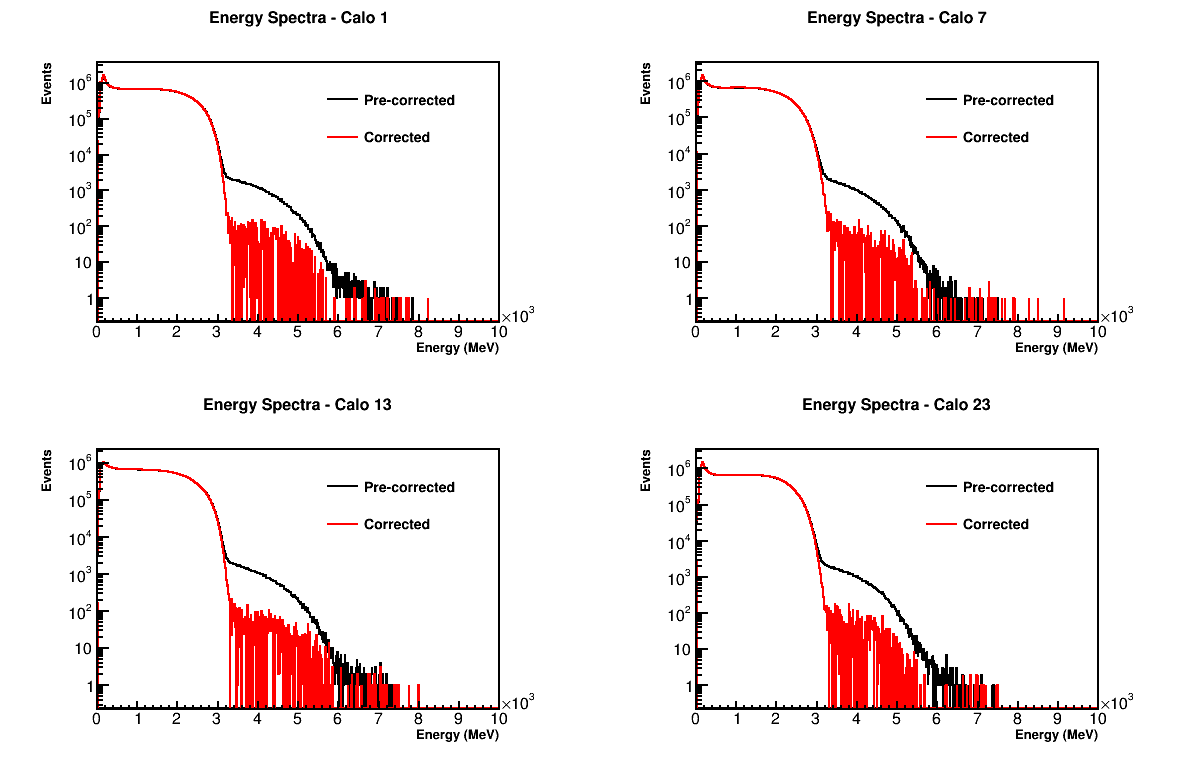
\includegraphics[width=\textwidth]{CaloEnergies}
    \caption[CaloEnergies]{Pre-corrected and corrected energy spectra for calorimeters 1, 7, 13, and 23 plotted on a log scale.}    
    \label{fig:CaloEnergies}
\end{figure}

\begin{figure}[]
	\centering
	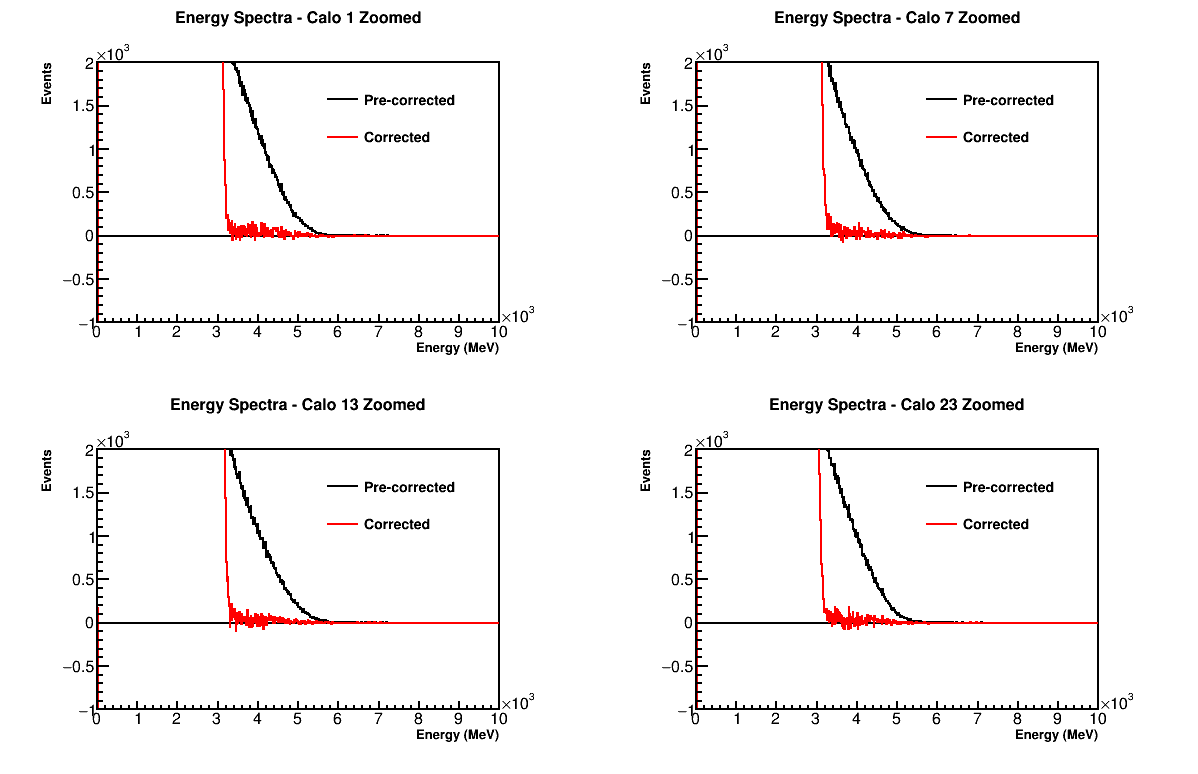
\includegraphics[width=\textwidth]{CaloEnergiesZoomed}
    \caption[CaloEnergiesZoomed]{Pre-corrected and corrected energy spectra for calorimeters 1, 7, 13, and 23 plotted on a linear scale and zoomed in.}    
    \label{fig:CaloEnergiesZoomed}
\end{figure}



\section{6 Parameter Ratio Fit}

\begin{figure}[H]
	\centering
	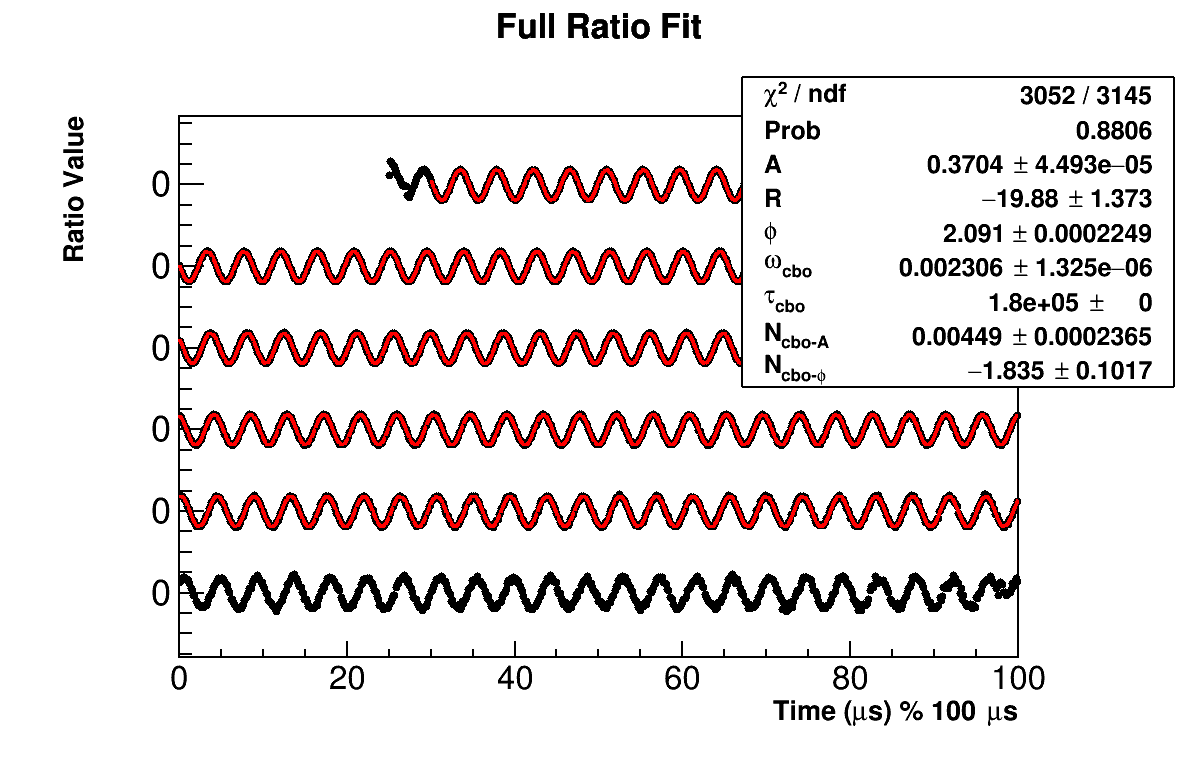
\includegraphics[width=\textwidth]{ratioCBO_moduloPlot}
    \caption[ratioCBO_moduloPlot]{Final fit result for the 60 hour dataset. The fit includes 6 free parameters and one fixed. The x axis is in units of $\mu$s modulo 100 $\mu$s, with successive portions of the data points and fit shifted downwards on the plot. The parameter values in the stats box for the CBO frequency and lifetime are in units of ns. R is blinded locally. The fit ranges from 30 $\mu$s to 500 $\mu$s.}
    \label{fig:ratioCBO_moduloPlot}
\end{figure}



\section{Residual and FFT}

\begin{figure}[H]
\centering
    \begin{subfigure}[]{0.45\textwidth}
	    \centering
		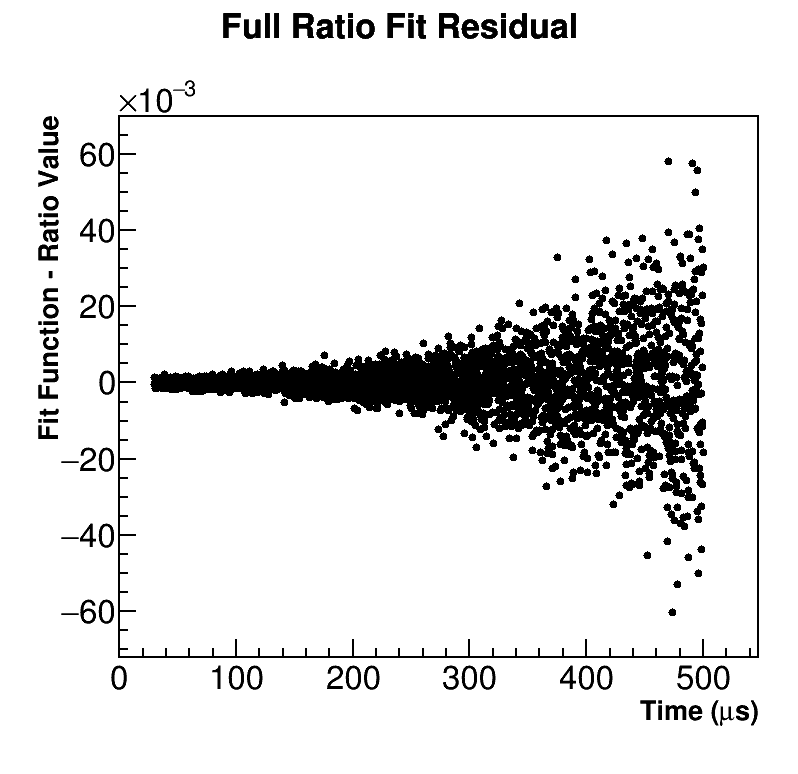
\includegraphics[width=\textwidth]{fitResidual}
	    \caption{Fit residuals.}
    \end{subfigure}
    \begin{subfigure}[]{0.45\textwidth}
	    \centering
		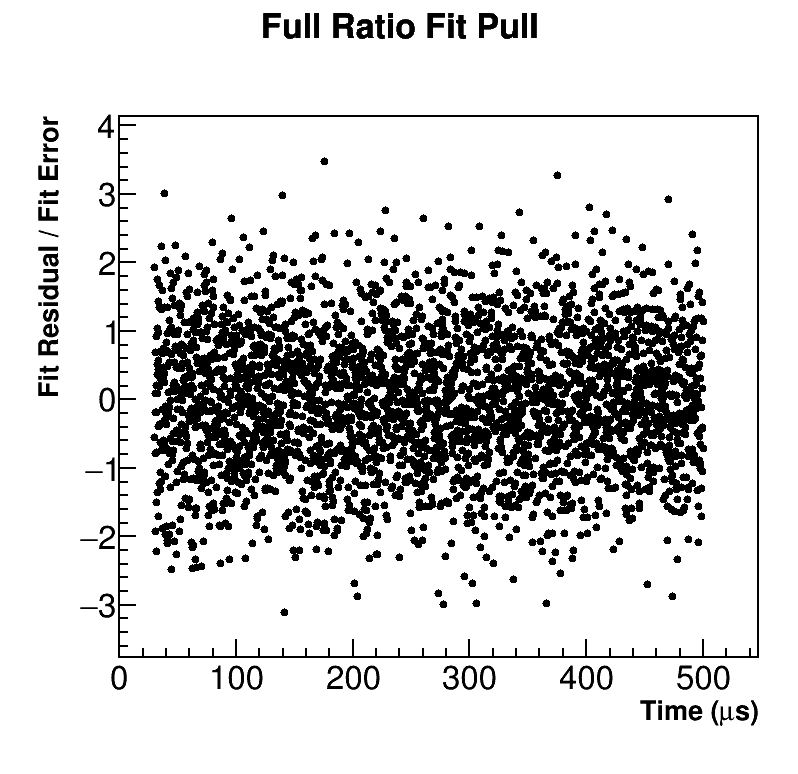
\includegraphics[width=\textwidth]{fitPull}
	    \caption{Fit pulls.}
    \end{subfigure}% %you need this % here to add spacing between subfigures
    \vspace{4mm}
    \begin{subfigure}[]{0.7\textwidth}
	    \centering
		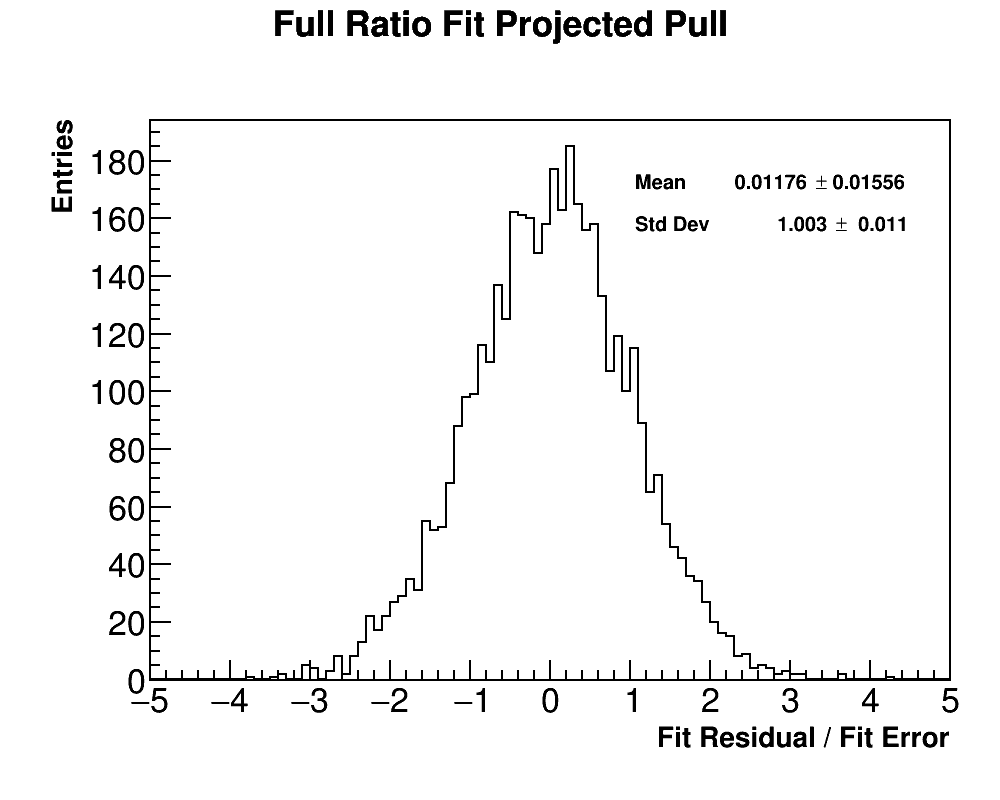
\includegraphics[width=\textwidth]{fitPull_projected}
	    \caption{Fit pulls projected onto the y axis. Note the Gaussian shape centered around 0 with unit width.}
    \end{subfigure}
\caption[fitResidual]{Residuals and pulls for the full ratio fit.}
\label{fig:fitResidual}
\end{figure}

\begin{figure}[]
	\centering
	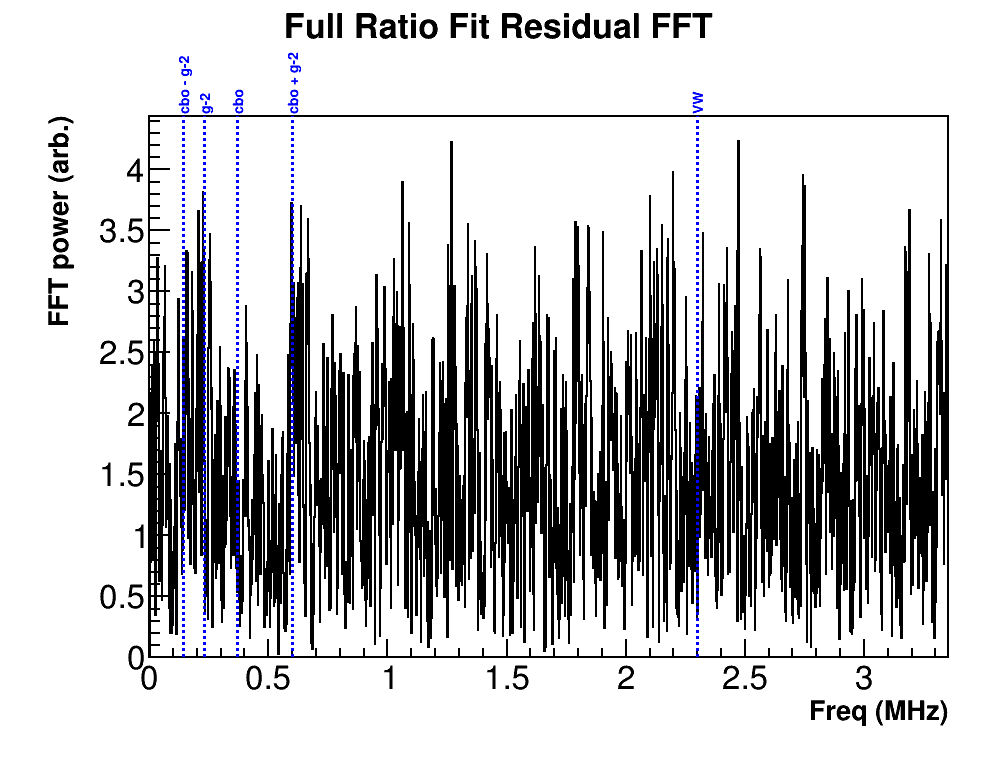
\includegraphics[width=\textwidth]{FFT_ratioCBOFit}
    \caption[FFT_ratioCBOFit]{FFT of the residuals of the full ratio fit. No significant peaks remain in the ratio fit residuals after fitting with CBO terms. Overlayed are dotted lines for the \gmtwo, CBO, and vertical waist frequencies. Peaks close to the lines are coincidental but don't line up when zoomed in.}
    \label{fig:FFT_ratioCBOFit}
\end{figure}

\begin{figure}[]
	\centering
	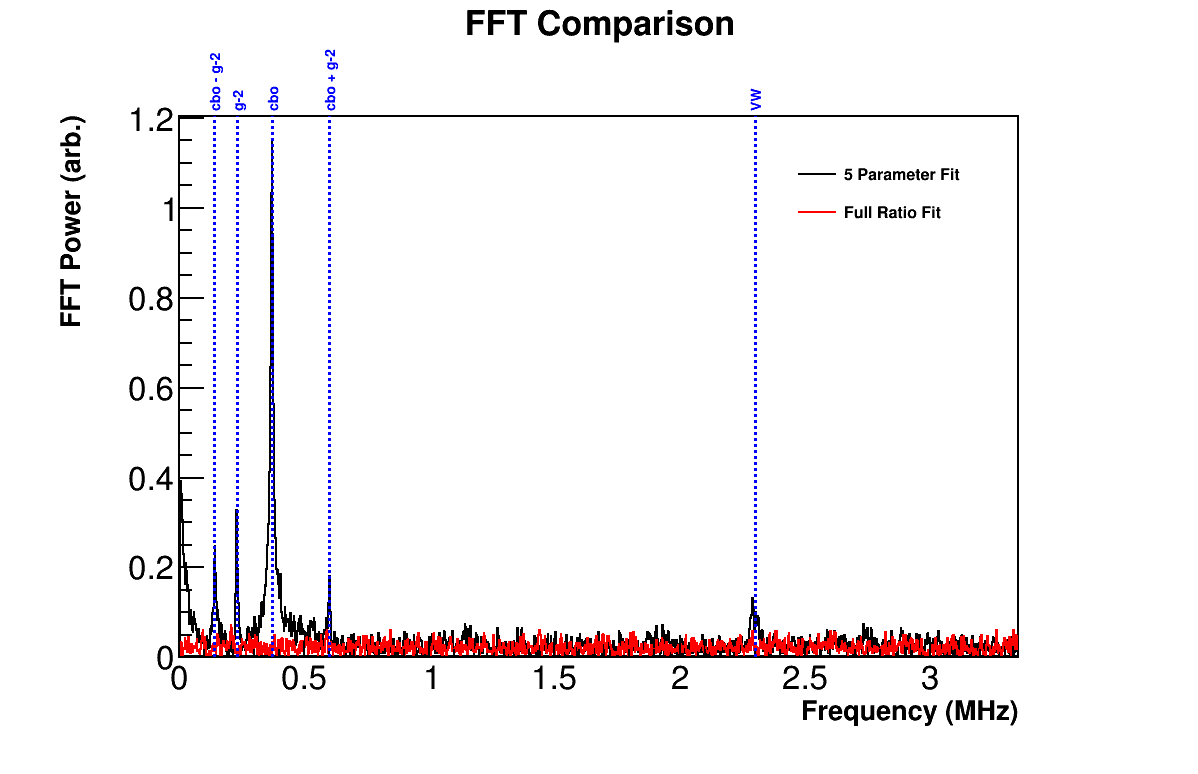
\includegraphics[width=\textwidth]{FFTComparison_RatioCBO}
    \caption[FFTComparison_RatioCBO]{A plot of the FFT of the residuals of the fit for the five parameter fit compared to the ratio fit. In black is the FFT for a five parameter fit, where peaks for the CBO and vertical waist can be seen as well as the \gmtwo peak. In red is the FFT of the full ratio fit residuals, where it has been scaled up to be visible on this plot.}
    \label{fig:FFTComparison_RatioCBO}
\end{figure}


\section{Start time scans}

\begin{figure}[H]
	\centering
	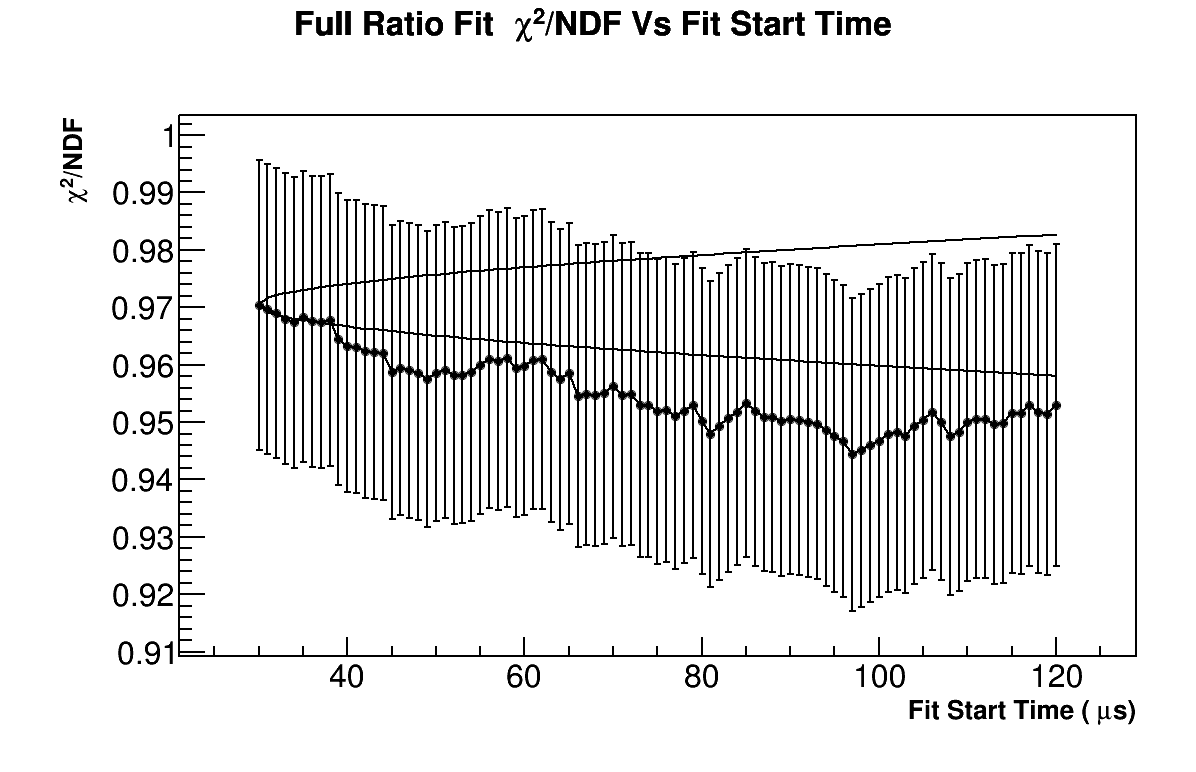
\includegraphics[width=\textwidth]{RatioCBO_Chi2NDF_Vs_FS_canv}
    \caption[RatioCBO_Chi2NDF_Vs_FS_canv]{Plotted is the \chisq per degree of freedom vs the start time of the fit. The solid lines indicate the one sigma statistically allowed difference in the fit result coming from the reduction in the data included in the fit. The error bars on the points are calculated as $\sqrt{2/NDF}$.}
    \label{fig:RatioCBO_Chi2NDF_Vs_FS_canv}
\end{figure}


\begin{figure}[]
\centering
    \begin{subfigure}[t]{0.45\textwidth}
	    \centering
		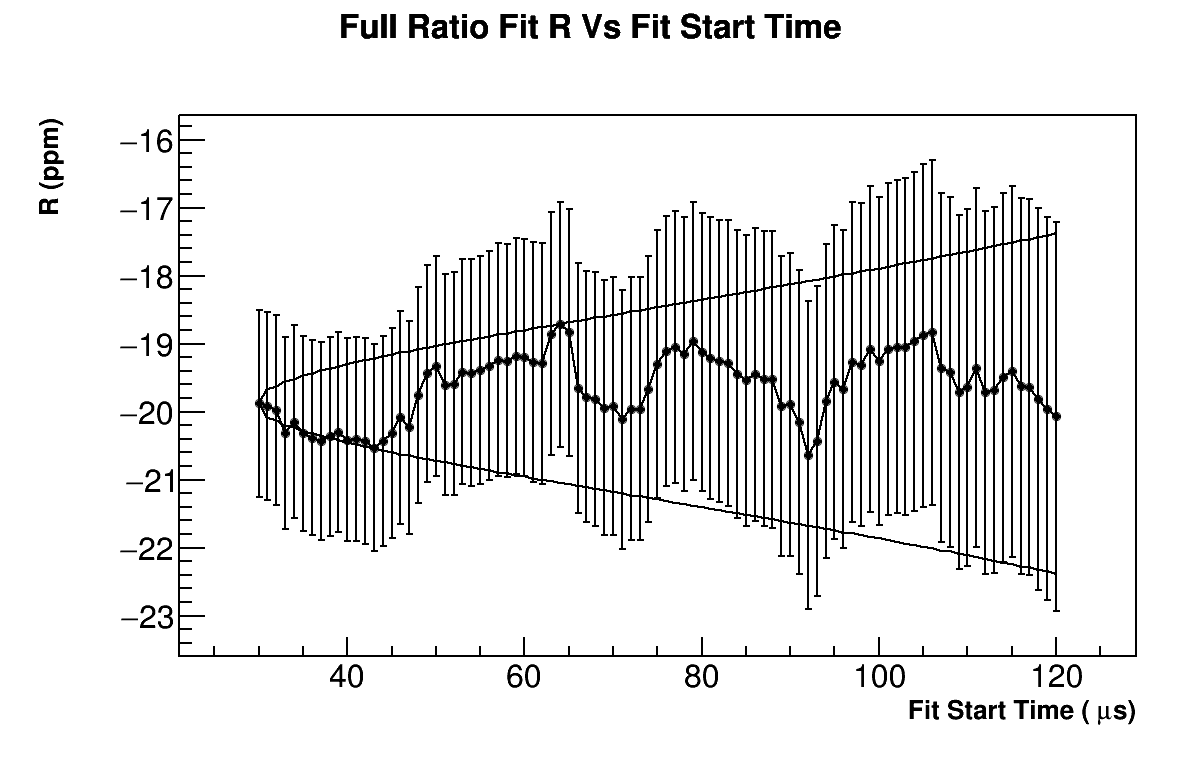
\includegraphics[width=\textwidth]{RatioCBO_R_FS_Canv}
	    \caption{Fitted R value vs fit start time.}
    \end{subfigure}
    \begin{subfigure}[t]{0.45\textwidth}
	    \centering
		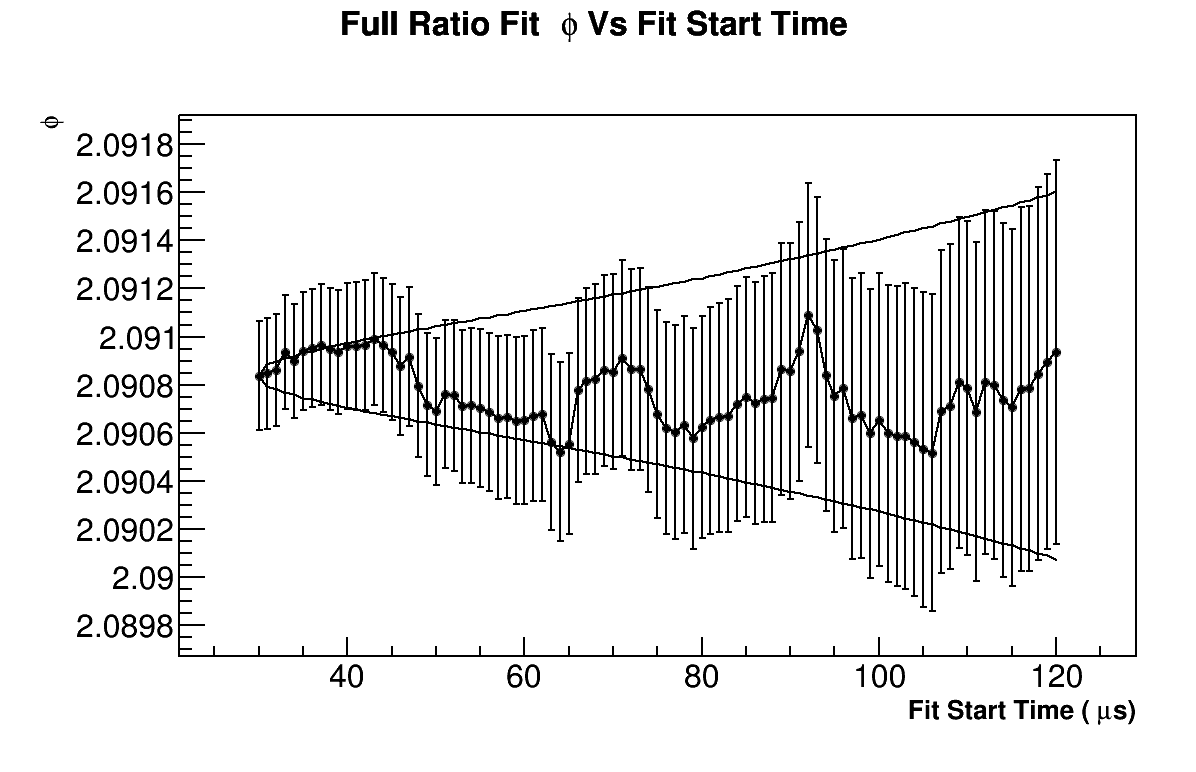
\includegraphics[width=\textwidth]{RatioCBO_phi_FS_Canv}
	    \caption{Fitted \gmtwo phase vs fit start time.}
    \end{subfigure}% %you need this % here to add spacing between subfigures
    \vspace{4mm}
    \begin{subfigure}[t]{0.45\textwidth}
	    \centering
		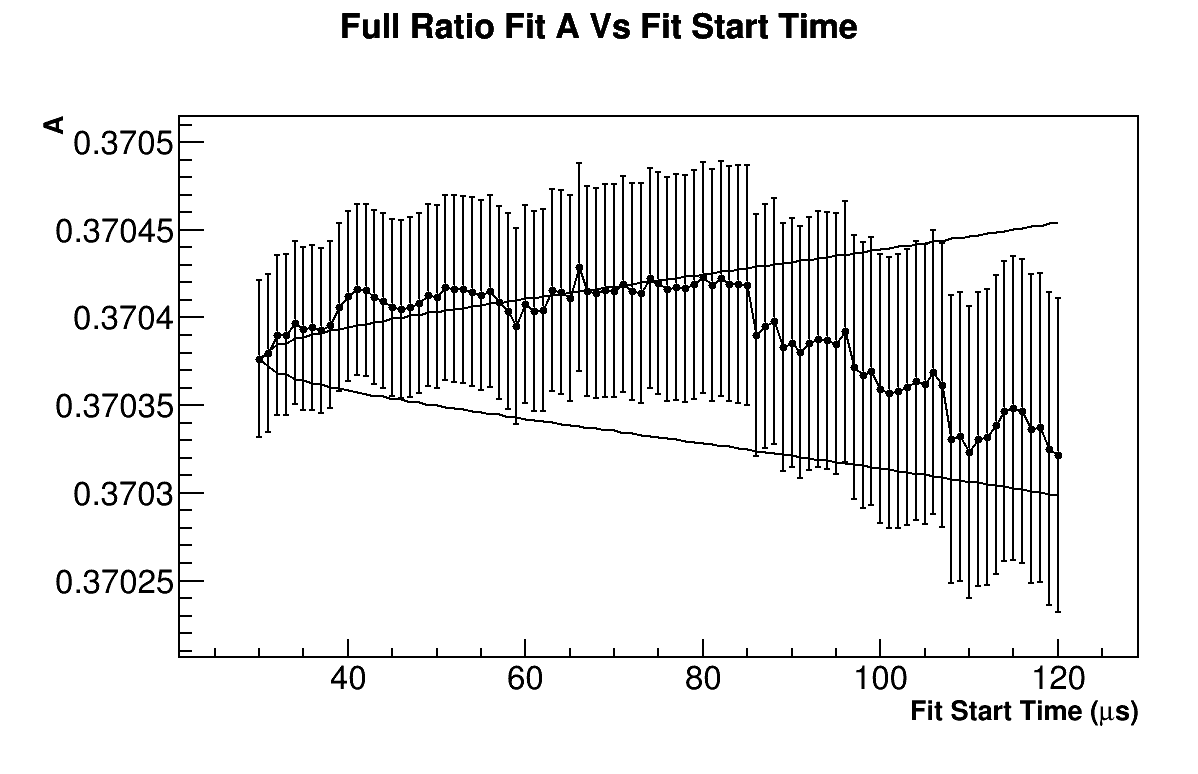
\includegraphics[width=\textwidth]{RatioCBO_A_FS_Canv}
	    \caption{Fitted asymmetry vs fit start time.}
    \end{subfigure}
    \begin{subfigure}[t]{0.45\textwidth}
	    \centering
		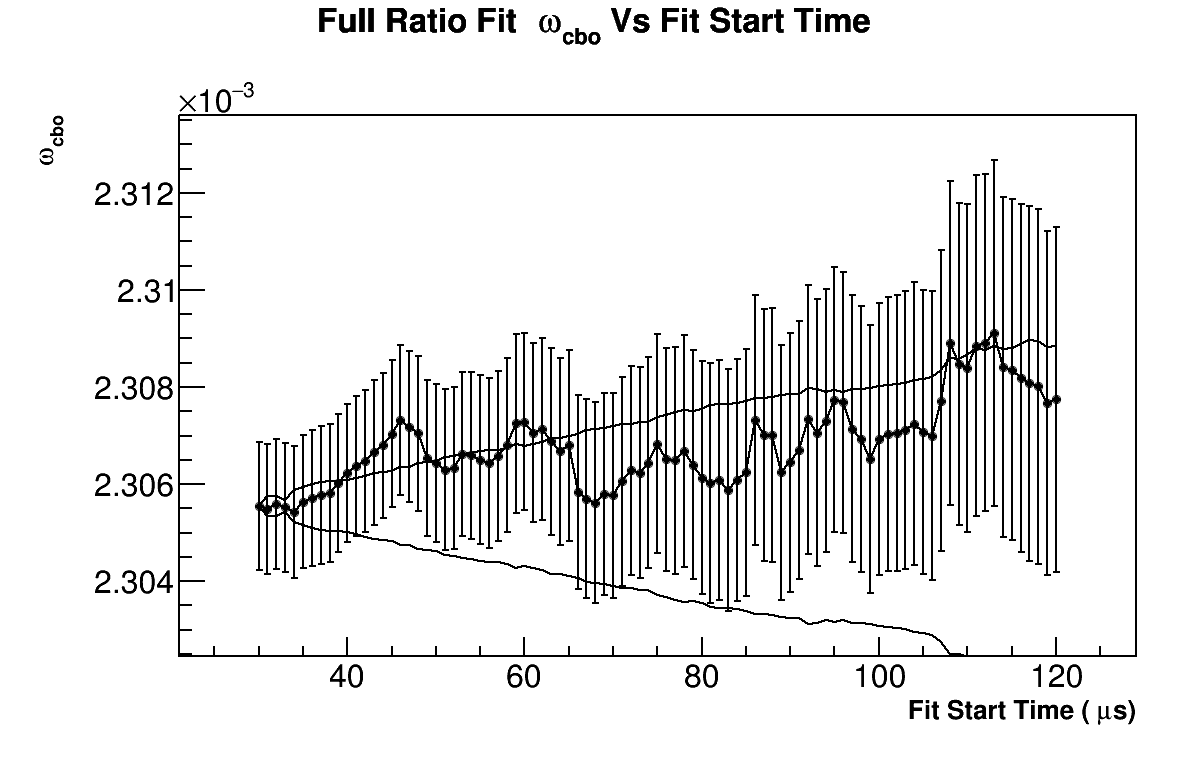
\includegraphics[width=\textwidth]{RatioCBO_omega_cbo_FS_Canv}
	    \caption{Fitted CBO frequency ($\omega_{0}$) vs fit start time.}
    \end{subfigure}% %you need this % here to add spacing between subfigures
    \vspace{4mm}
    \begin{subfigure}[t]{0.45\textwidth}
	    \centering
		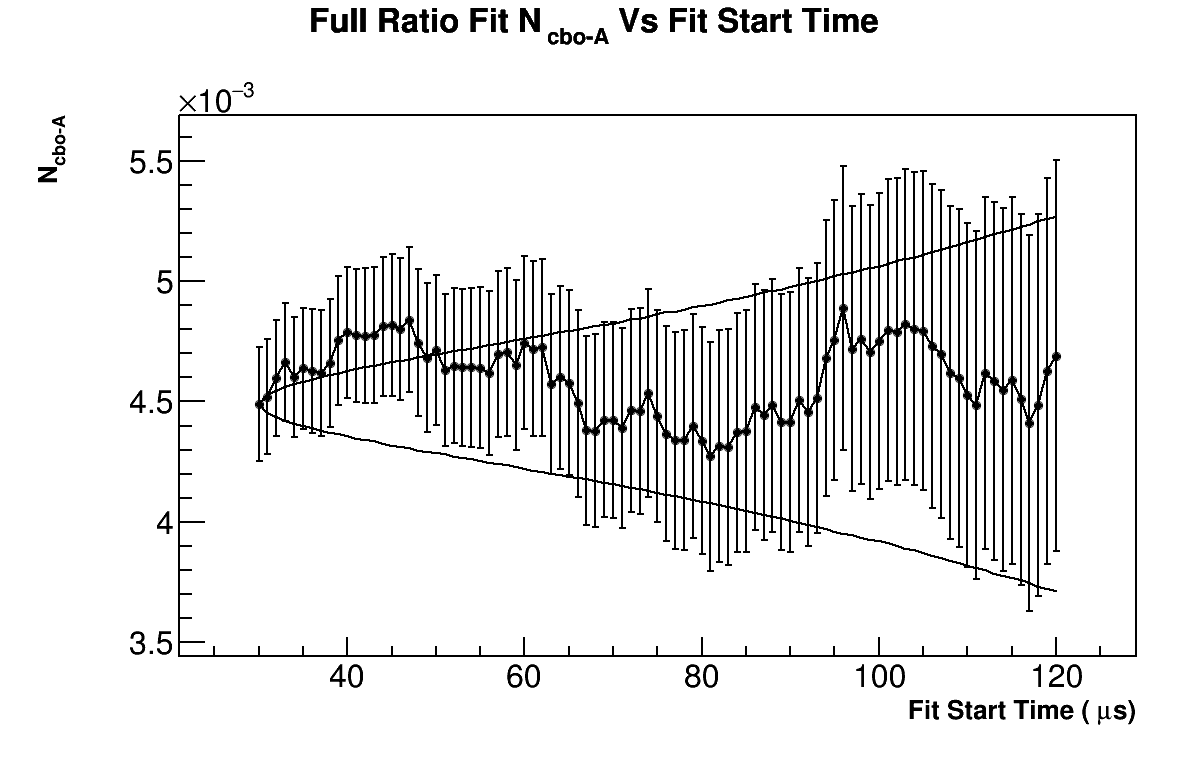
\includegraphics[width=\textwidth]{RatioCBO_N_cbo-A_FS_Canv}
	    \caption{Fitted CBO amplitdue vs fit start time.}
    \end{subfigure}
    \begin{subfigure}[t]{0.45\textwidth}
	    \centering
		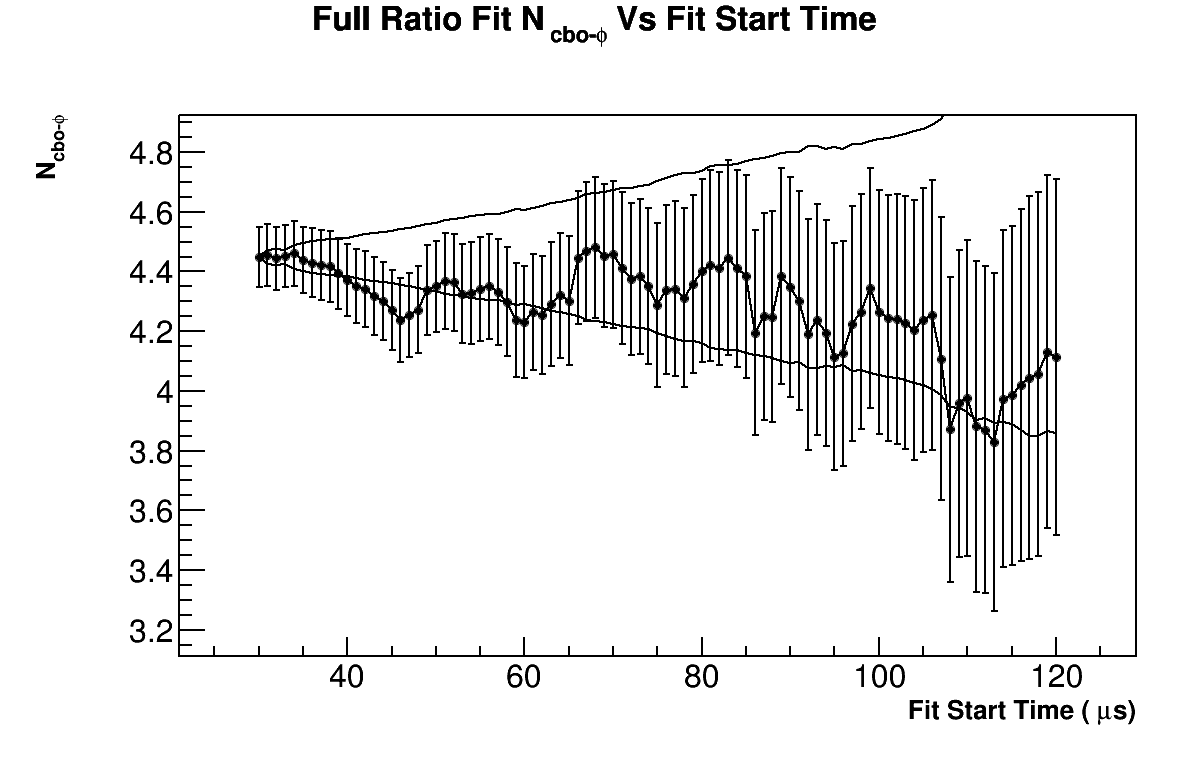
\includegraphics[width=\textwidth]{RatioCBO_N_cbo-phi_FS_Canv}
	    \caption{Fitted CBO phase vs fit start time.}
    \end{subfigure}% %you need this % here to add spacing between subfigures
\caption[FitStartScans]{Start time scans for the free parameters in the full ratio fit. All parameters are consistently within the one sigma statistical bands.}
\label{fig:FitStartScans}
\end{figure}

\section{Stop time scans}

I can produce stop time scans, and the results are consistent with the statistical significance bands, but some of the fits aren't perfect leading to some bad looking plots. Should I leave these out completely? Play more with the limits like I did to get the start time scans clean? Hack the plotting module to produce nicer looking plots? Or only include the good looking plots like R and the chi2?


\section{Results vs calorimeter}

\begin{figure}[H]
	\centering
	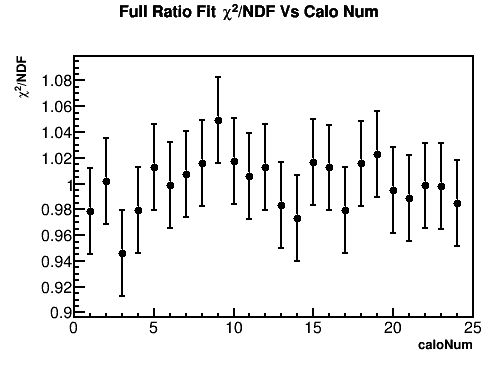
\includegraphics[width=.7\textwidth]{RatioCBOFit_Chi2NDF_Vs_Calo_Canv}
    \caption[RatioCBOFit_Chi2NDF_Vs_Calo_Canv]{Plotted is the \chisq per degree of freedom vs calorimeter number.}
    \label{fig:RatioCBOFit_Chi2NDF_Vs_Calo_Canv}
\end{figure}


\begin{figure}[H]
\centering
    \begin{subfigure}[t]{0.4\textwidth}
	    \centering
		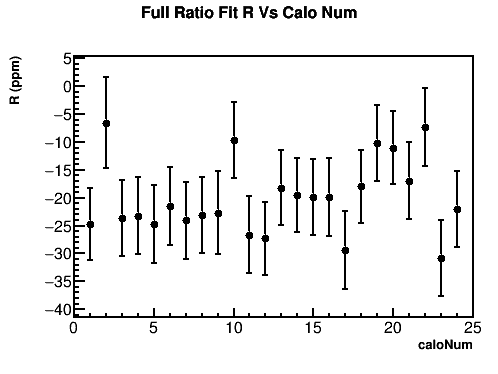
\includegraphics[width=\textwidth]{RatioCBOFit_R_Vs_Calo_Canv}
	    \caption{Fitted R value vs calorimeter number.}
    \end{subfigure}
    \hspace{4mm}
    \begin{subfigure}[t]{0.4\textwidth}
	    \centering
		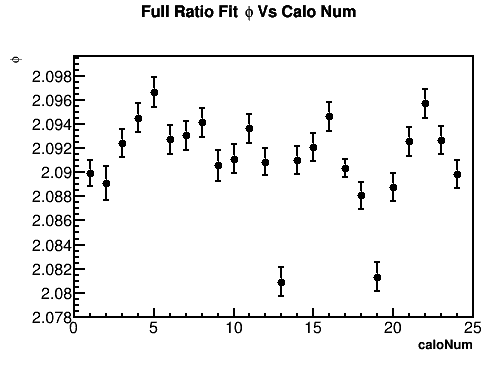
\includegraphics[width=\textwidth]{RatioCBOFit_phi_Vs_Calo_Canv}
	    \caption{Fitted \gmtwo phase vs calorimeter number. Calorimeters 13 and 19 lie behind the trackers leading to the different \gmtwo phases.}
    \end{subfigure}% %you need this % here to add spacing between subfigures
    \vspace{4mm}
    \begin{subfigure}[t]{0.4\textwidth}
	    \centering
		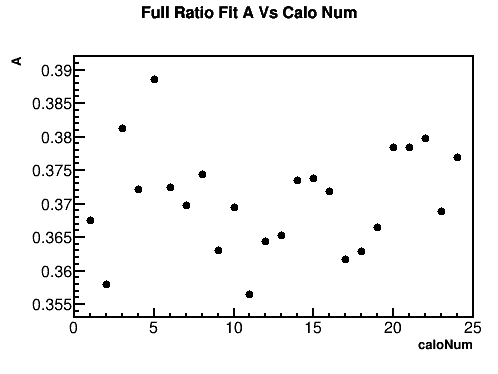
\includegraphics[width=\textwidth]{RatioCBOFit_A_Vs_Calo_Canv}
	    \caption{Fitted asymmetry vs calorimeter number.}
    \end{subfigure}
    \hspace{4mm}
    \begin{subfigure}[t]{0.4\textwidth}
	    \centering
		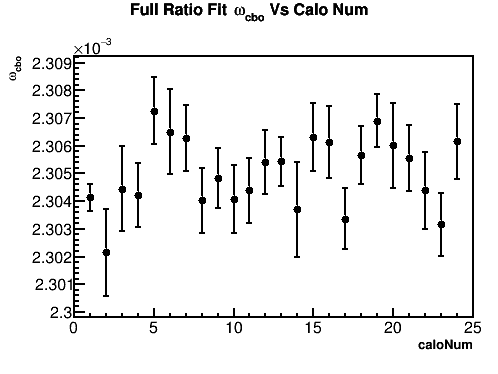
\includegraphics[width=\textwidth]{RatioCBOFit_omega_cbo_Vs_Calo_Canv}
	    \caption{Fitted CBO frequency ($\omega_{0}$) vs calorimeter number.}
    \end{subfigure}% %you need this % here to add spacing between subfigures
    \vspace{4mm}
    \begin{subfigure}[t]{0.4\textwidth}
	    \centering
		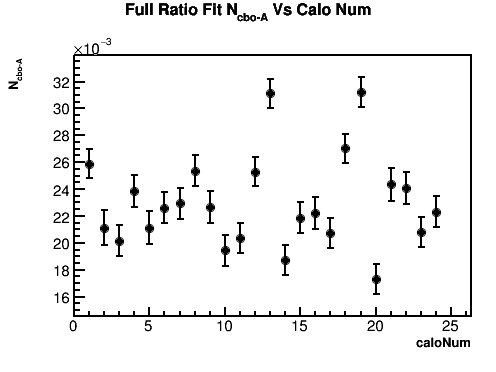
\includegraphics[width=\textwidth]{RatioCBOFit_N_cbo-A_Vs_Calo_Canv}
	    \caption{Fitted CBO amplitdue vs calorimeter number.}
    \end{subfigure}
    \hspace{4mm}
    \begin{subfigure}[t]{0.4\textwidth}
	    \centering
		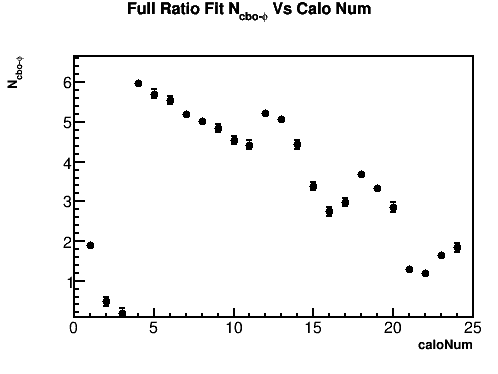
\includegraphics[width=\textwidth]{RatioCBOFit_N_cbo-phi_Vs_Calo_Canv}
	    \caption{Fitted CBO phase vs calorimeter number. The CBO phase varies from 0 to 2$\pi$ around the ring.}
    \end{subfigure}% %you need this % here to add spacing between subfigures
\caption[PerCaloPlots]{Full ratio fit parameter values vs calorimeter number.}
\label{fig:PerCaloPlots}
\end{figure}


\section{Correlation matrix for fit parameters}

\begin{table}[H]
\setlength\tabcolsep{0pt}
\begin{tabular*}{\linewidth}{@{\extracolsep{\fill}}lLBLLLLL{c}}
% \begin{tabular*}{\linewidth}{@{\extracolsep{\fill}}lL>{\boldmath\bfseries}LLLLLL{c}}
  \toprule
            & \thead{$A$} & \thead{$R$} & \thead{$\phi$} & \thead{$\omega_{cbo}$} & \thead{$\tau_{cbo}$ (fixed)} & \thead{$N_{cbo-A}$} & \thead{$N_{cbo-\phi}$} \\
  \midrule
	$A$    			 	 &  1.0000  &  0.0049  & -0.0068  & -0.0166  &  0.0000  & -0.0098  &  0.0233  \\
	$R$     			 &  0.0049  &  1.0000  & -0.8300  & -0.0204  &  0.0000  &  0.0207  &  0.0282  \\
	$\phi$   			 & -0.0068  & -0.8300  &  1.0000  &  0.0280  &  0.0000  & -0.0287  & -0.0387  \\
	$\omega_{cbo}$   	 & -0.0166  & -0.0204  &  0.0280  &  1.0000  &  0.0000  &  0.0773  & -0.8585  \\
	$\tau_{cbo}$ (fixed) &  0.0000  &  0.0000  &  0.0000  &  0.0000  &  1.0000  &  0.0000  &  0.0000  \\
	$N_{cbo-A}$   	 	 & -0.0098  &  0.0207  & -0.0287  &  0.0773  &  0.0000  &  1.0000  & -0.0656  \\
	$N_{cbo-\phi}$   	 &  0.0233  &  0.0282  & -0.0387  & -0.8585  &  0.0000  & -0.0656  &  1.0000  \\
  \bottomrule
\end{tabular*}
\caption{Correlation matrix for the full ratio fit. The CBO lifetime is fixed but included in this table. The only significant correlation to R is the \gmtwo phase.}
\end{table}



